\title{Lecture week 6}
\maketitle
\section{11. feb}
\subsection*{Transversatility}
Machine for making manifolds.
\newline Take a smooth map $f: X \to Y \left(f:\R^n \to \R^m\right)$.
\newline Find a regular value $y\in Y$. Then $f ^{-1}(y) \subseteq X $ is a manifold.

\subsection*{Question:}
If $p: \R^2 \to \R$ a polynomial $p(x,y)$ and $a\in \R$ a regular value of $p$. Then $p ^{-1}(a) \subseteq \R^n $ is a manifold. Which one?

\subsection*{How to describe a 1-manifold?}
Connected $1$-manifold: diffeo to $\R$ or $S^1$ (these are the only possibilities)
\newline In general a $1$-manifold is a disjoint union of $\R$'s and $S^1$'s.

\subsection*{Hornack's inequality}:
If $p: \R^2 \to \R$ polynomial, $deg(p)=m, a\in R$ a regular value of $p$, then $p ^{-1}(a)=\{(x,y)\in \R^2 | p(x,y)=a\}$ has at most
  $$\frac{(m-1)(m-2)}{2}+1$$
connected components.

\subsection*{Transversatility}
Let $f: X \to Y$ be a smooth map and $Z \subseteq Y$ a smooth manifold, when is $f ^{-1} (Z) \subseteq X $ a smooth manifold?
\newline We first study one point at the time. Consider $x\in f ^{-1}(Z)$. We'll see how we can find an open set about $x\in f ^{-1}(Z)$ that's ``euclidean''.
\newline Consider $x\in f ^{-1}(Z)$, say $y\in f(x)$.
\newline Find $g:V\to \R^2$ so that $g ^{-1}(0)=V\cap Z$, $0$ a regular value of $g$. Observe taht $f ^{-1}(V)=u \subseteq X $ open so $u \cap f ^{-1}(Z)$ open rel. $f ^{-1}(Z)$. Now we can compose
  $$g\circ f: u \to \R^2, f ^{-1}(Z\cap V)=f ^{-1}(g ^{-1}(0))=(g\circ f)^{-1}(0)$$
Question, is $0$ a regular value of $g\circ f$? If so $\Rightarrow u \cap f ^{-1} (Z)$ is a manifold?
\newline When is $0$ a regular value of $g\circ f$? At the very least when is $D(g\circ f)x$ surjective? Which will give $f ^{-1}(Z)\cap u$ locally euclidean at $x$.
\newline So $0$ is a regular value of $g$, so $D_{gy}$ is surjective.
\newline $D(g\circ f)_x$ surjective if $Df_x$ is surjecive. This is however overkill.
\newline Necessary and sufficient condition is that
  $$Image(Df_x)+Ker(Dg_y)=T_yY$$
  $g: u \to \R^l, g ^{-1}(0)=z\cap u$ submanifold and $0$ regular value
    $$\Rightarrow T_{yg}^{-1}(0)=Ker(Dg_y)$$
Then $f ^{-1}(Z)$ will be a manifold at $x$ if $Image(Df_x)+T_yZ=T_yY$. (entirely dependent on $f$ and $Z$).

\begin{definition}
  We say a map $f: X \to Y$ is transverse to $Z \subseteq Y$ (a submanifold) if at all $f(x)=y$, $x\in f ^{-1}(Z) \Rightarrow Image(Df_x)+T_yZ=T_yY$.
\end{definition}
\begin{theorem}
  If $f: X \to Y$ is transverse to $Z \subseteq Y$, then $f ^{-1}(Z)$ is a manifold.
\end{theorem}
\begin{proof}
  Basically the argument before the definition.
\end{proof}

\begin{remark}
  $Codim_YZ=dim Y - dim Z$
\end{remark}
\begin{corollary}
  $$codim_xf ^{-1}(Z)= codim_Y Z.$$
\end{corollary}
\begin{proof}
  $dim Z= dim Y - l, dim f ^{-1}(Z)=dim ((g\circ f) ^{-1}(0))=dim X-l$
  $$\Rightarrow l = codim_YZ, l=codim_X f ^{-1}(Z)$$
\end{proof}

\begin{definition}
  Notation:
    $$f \transv Z= f\text{ is transverse to } Z.$$
\end{definition}
\begin{example}
  $f: \R \to \R, f(x)=x^n, df =
\begin{bmatrix}
  nx^{n-1}
\end{bmatrix}
  $ is $f \transv \{0\}$? We know $T_0\{0\}=\{0\}$ which is equivalent to $\transv \Leftrightarrow df_0$ surjective. This only happens when $n=1$. When $Z=\{y\}, \transv \Leftrightarrow  y$ a regular value.
\end{example}
\begin{example}
  $$\Gamma(f)(x)=(x, x^n)$$
  $$z= \{(x,0)| x\in \R\}=\R\times \{0\}$$
  $$\Gamma(f)^{-1}(Z) \Leftrightarrow \{x\in \R | f(x)=0\}$$
  This is an intersection problem. $\Gamma(f)$ not transverse to $Z$.
  \begin{center}
  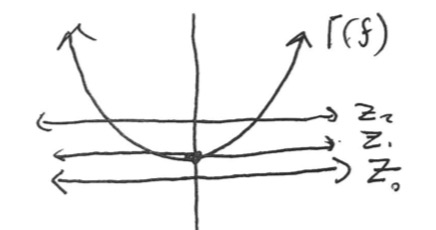
\includegraphics[width=0.30\paperwidth]{vaar2020/difftop/week06/gammaf}
  \end{center}
  $$\Gamma(f)^{-1}(Z)=\{x| x^n = 0\} \Leftrightarrow \{(x,x^n) | x\in \R\} \cap \{(x,0)| x\in \R\}$$
  $$\Gamma(f)\cap z_0= \emptyset$$
  $$\Gamma(f) \cap z_1\neq \emptyset$$
  $$\Gamma(f)\cap z_2 \neq 0$$

\end{example}

\section{13. feb.}
\begin{itemize}
  \item Homotopy and stability
  \item Don't use the entire week on the midterm
\end{itemize}
\begin{definition}
  Let $f_0 : X\to Y$ and $f_1: X\to Y$ be two smooth functions. We say $f_0 \sim f_1$, in words, \emph{$f_0$ is homotopic to $f_1$}, if there exists smooth $F: X \times [0,1] \to Y$ with $F(x,0)=f_0(x)$ and $F(x,1)=f_1(x)$. We'll use $f_t : X\to Y, f_t(x)=F(x,t)$. We'll think of $F$ as a family of maps $f_t : X\to Y$ deforms $f_0 $ into $f_1$.
\end{definition}
\begin{example}
  $X=\R^0$ and $Y=\R^2$, $f: \R^0 \to \R^2$, picks at $x_0 = f(0), g: \R^0 \to \R^2, x_1=g(0)$
  \newline $\Rightarrow f\sim g$, if there is $F:\{0\} \times [0,1] \to \R^2$.
  \newline $F(0,t)\in \R^2, F(0,0)=x_0$ and $F(0,1)=x_1$. Alternate name for this case: $x_0$ and $x_1$ are in the same path component of $X$ if $x_0 \sim x_1$.
\end{example}
\begin{exercise}
      $X$ a manifold, $X$ is connected, $iff \forall x_0,x_1 \in X, x_0 \sim x_1$.
\end{exercise}
In $\R^2$, any teo points $x_0, x_1 \in \R^2$ are connected by $F(t)=x_0+t(x_1-x_0), t\in \R, F(0)=x_0, F(1)=x_1$.
\begin{proposition}
  Let $f: X\to \R^n$ be any smooth map. Then $f$ is homotopic to $0: X \to \R^n; x\mapsto 0$.
\end{proposition}
\begin{proof}
  $F(x,t)=(1-t)f(x), F: X\times \R \to \R^n, F(x,0)=f(x), F(x,1)=0$.
\end{proof}
\begin{center}
      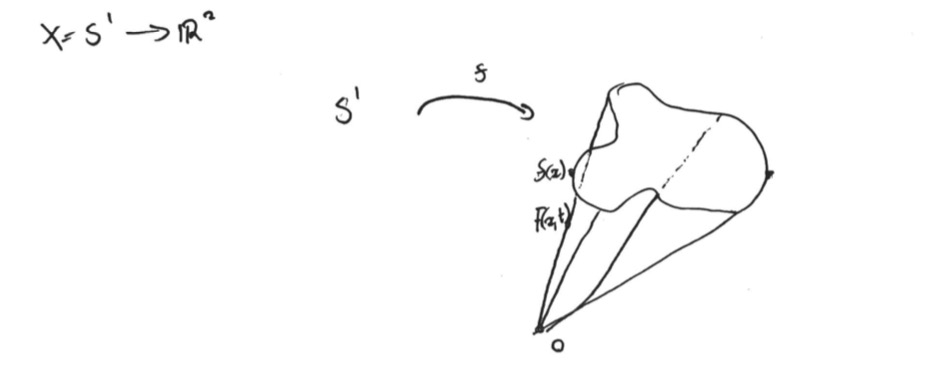
\includegraphics[width=0.30\paperwidth]{vaar2020/difftop/week06/s1toR2}
\end{center}
\begin{example}
  $f:S^1\to \R^2\setminus\{0\}: (x,y)\mapsto (x,y)$.
  \newline $f$ is not homotopic to any constant map.
\end{example}
\begin{definition}
  Two manifolds, $X,Y$ are (smoothly) homotopy equivalent if we can find $f: X\to Y, g:Y \to X$ so that $g\circ f \sim id_X$ and $f \sim g = id_Y$. We say \emph{$g$ is the homotopy inverse of $f$}.
\end{definition}
\begin{definition}
  A manifold $X$ is contractable if $X$ is homotopy equivalent to a point $(\R^0)$.
\end{definition}

$X$ is contractable if we have
\begin{center}
    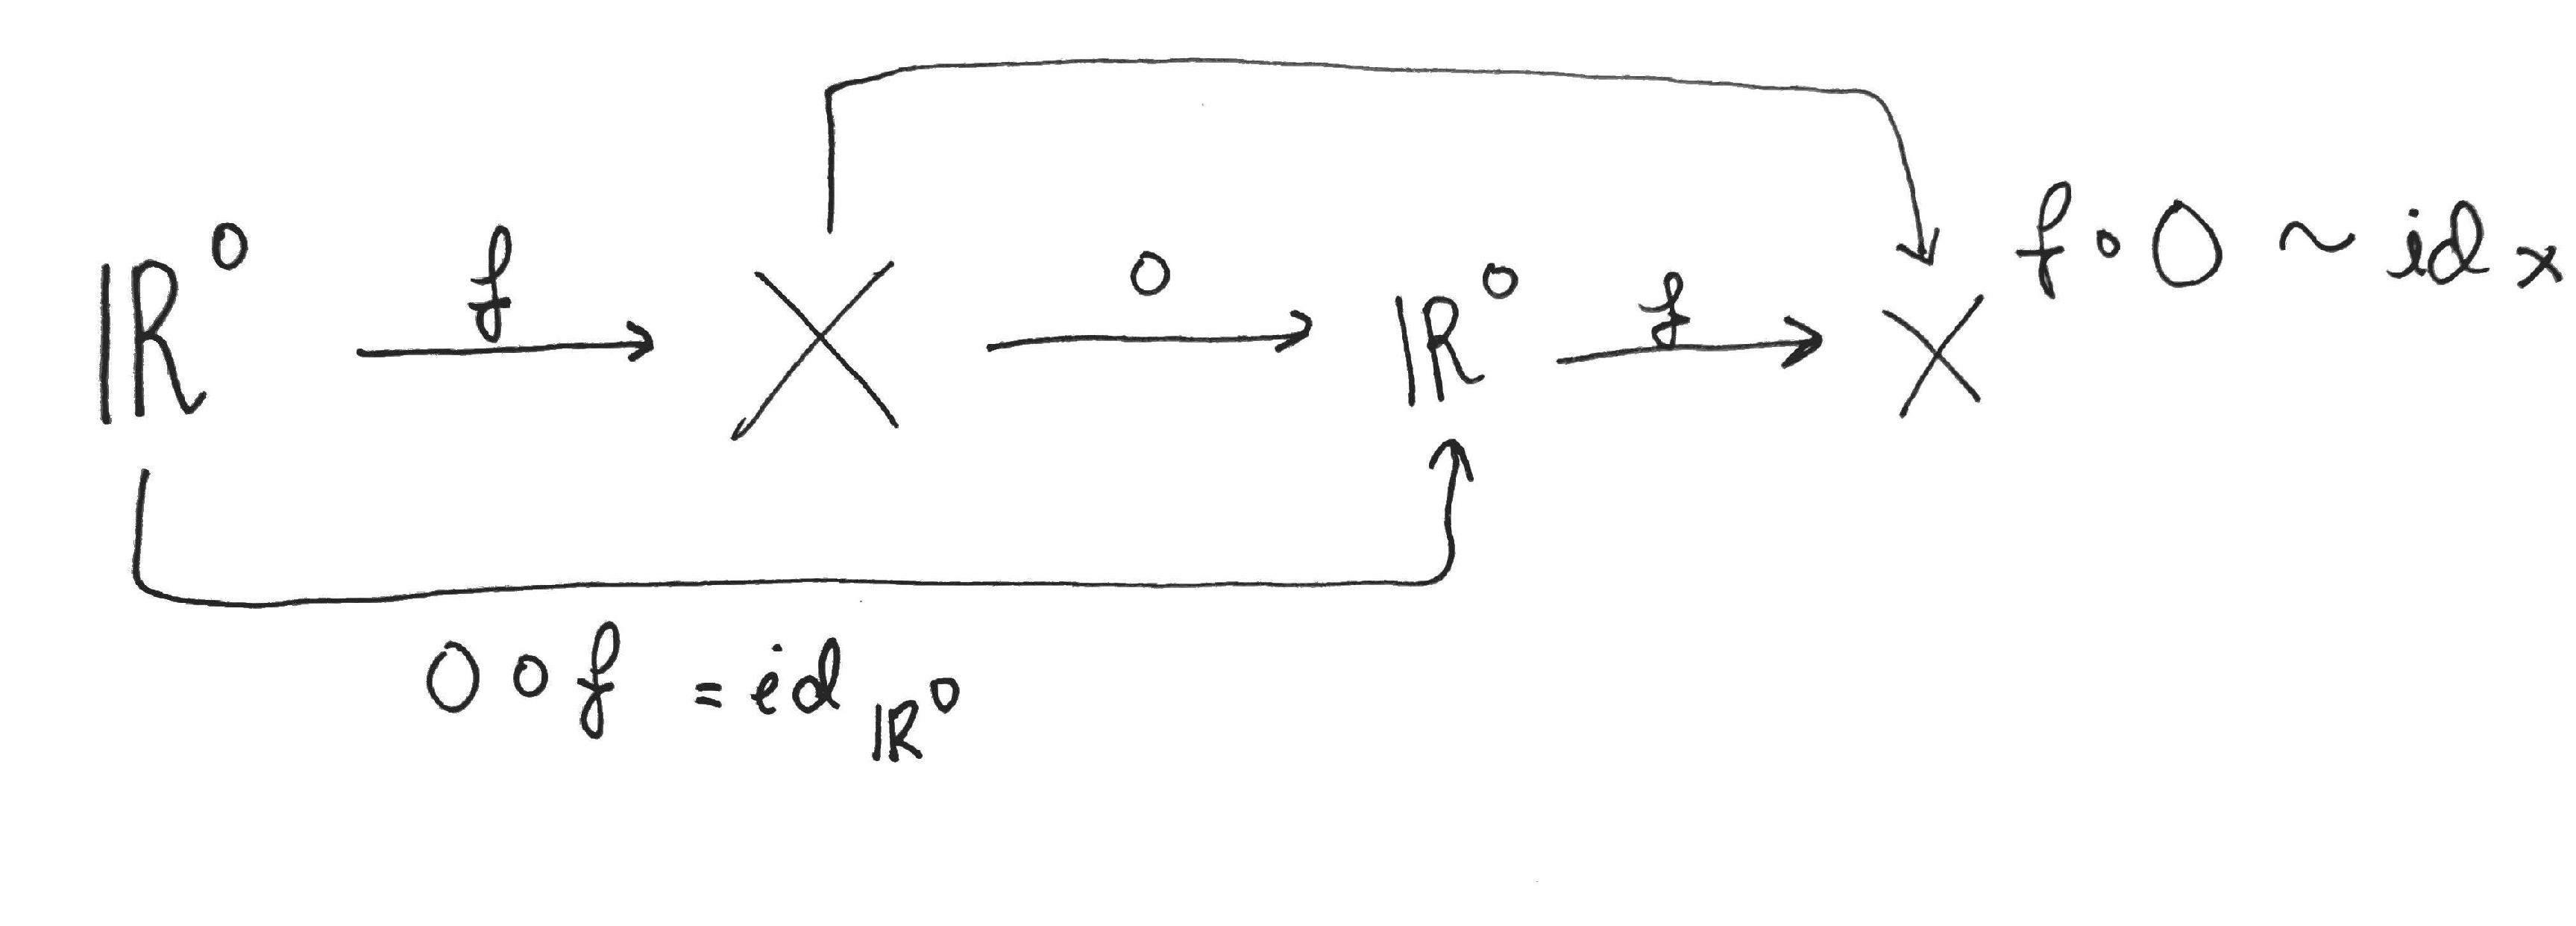
\includegraphics[width=0.40\paperwidth]{vaar2020/difftop/week06/contraction}
\end{center}
$f \circ 0(x)= f(0)=x_0 \in X$, we need a homotopy
\newline $F: X\times[0,1] \to X$, $F(x,0)=x$ and $F(x,1)=x_0$

\begin{proposition}
  $\R^n$ is contractable
\end{proposition}
\begin{proof}
  $id: \R^n \to \R^n$ is homotopic to $0: \R^n \to \R^n$. ``Straight line homotopy'' $F(x,t)=(1-t)x$.
    \qedhere
\end{proof}
$$\R^n \sim \R^0 , \forall n$$

\begin{notation}
  $C^{\infty}(X,Y)$ is the set of all smooth maps $f: X \to Y$ .
\end{notation}
\begin{remark}
  Homotopy is an equivalence relation on $C^{\infty}(X,Y)$.
\end{remark}

  \begin{center}
    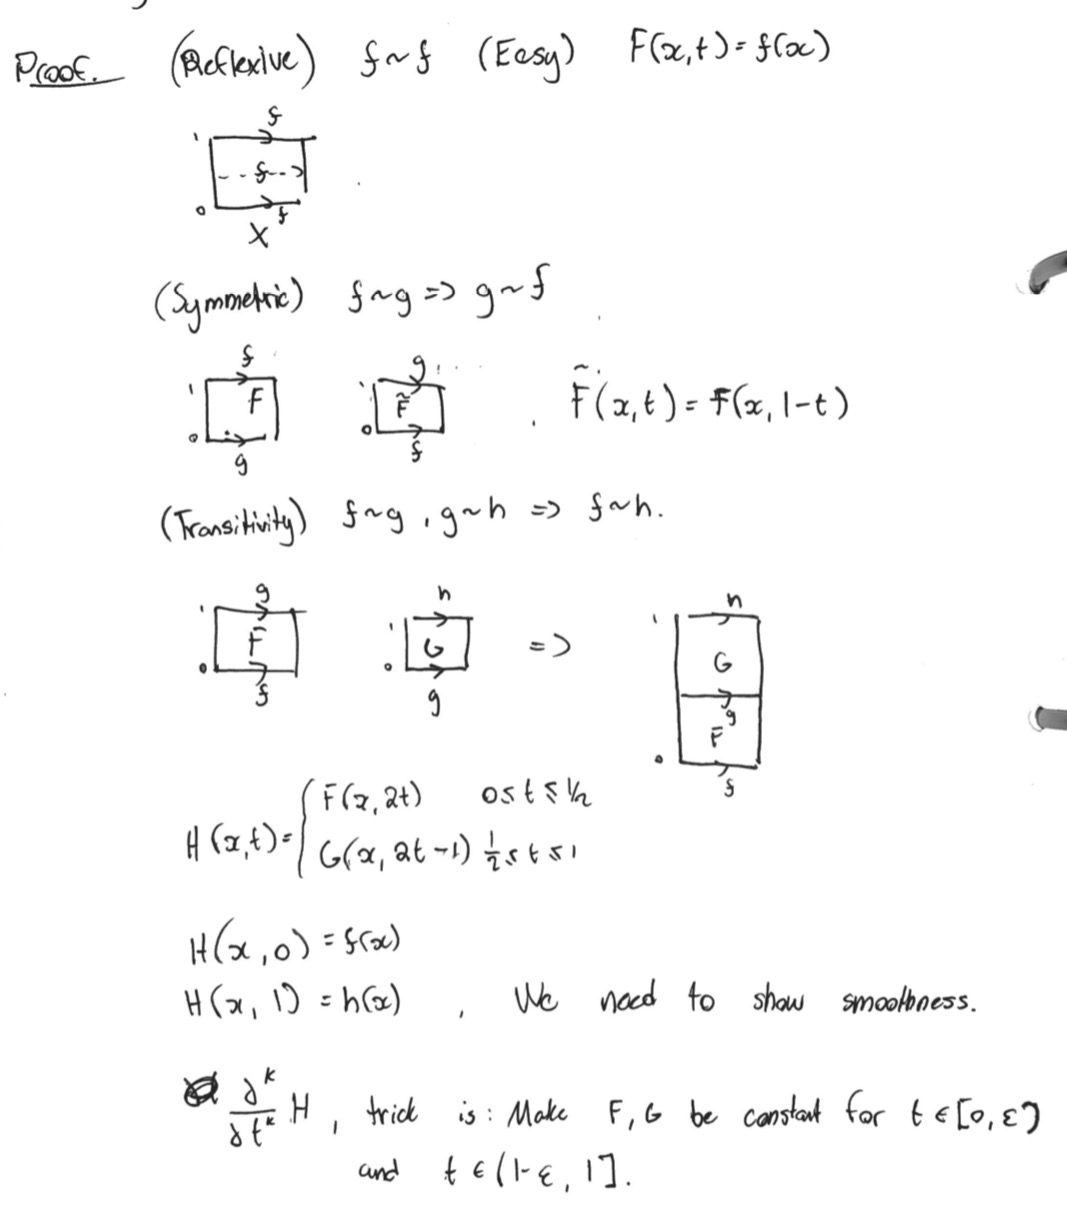
\includegraphics[width=0.40\paperwidth]{vaar2020/difftop/week06/equivrel}
    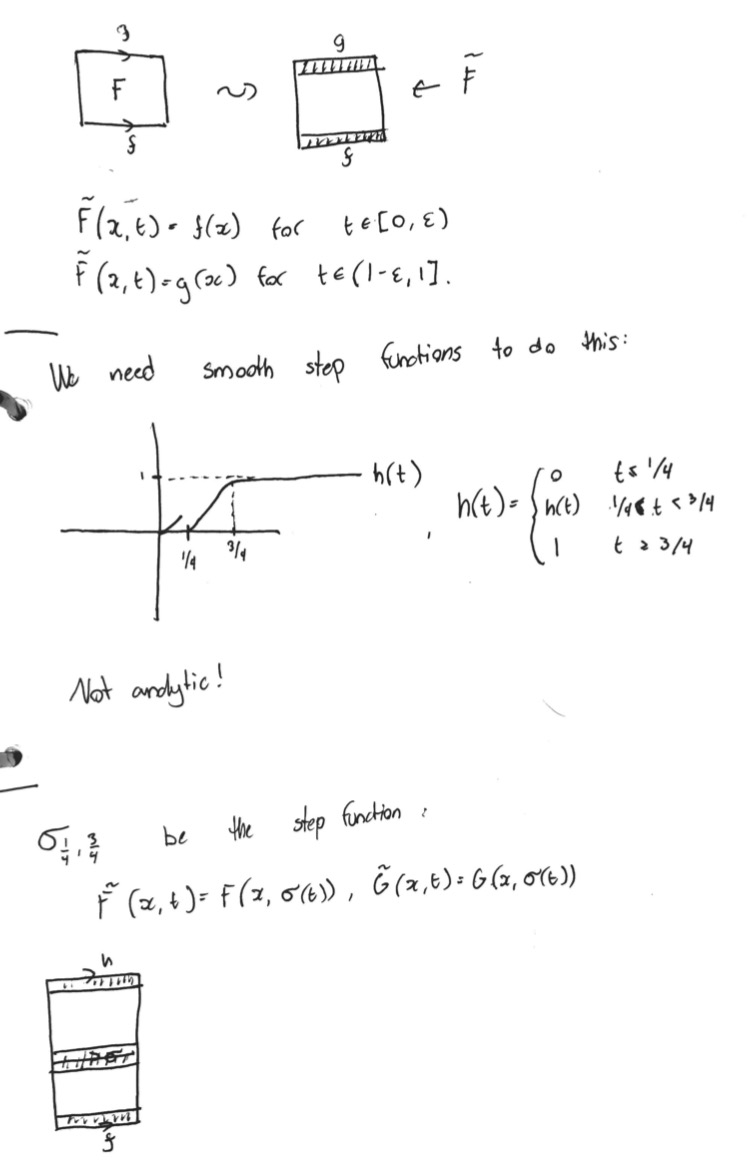
\includegraphics[width=0.40\paperwidth]{vaar2020/difftop/week06/equivrel2}
  \end{center}

\begin{definition}
  A class of maps $\mathcal{T} \subseteq C^{\infty}(X,Y)$ is \emph{stable} if for any homotopy $F: X \times I \to Y$ with $f_0 \in \mathcal{T}$ there exists $\varepsilon >0$ so $f_t \in \mathcal{T} \forall t <\varepsilon$.
\end{definition}
\begin{example}
  $\mathcal{T}=\{f: \R^1 \to \R^2 | f(\R^1) \cap \{(x,0) | x\in \R \} \neq \emptyset \}$ Stable family?
    \begin{center}
      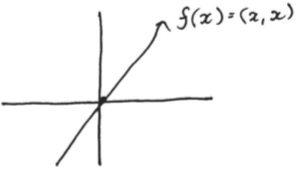
\includegraphics[width=0.30\paperwidth]{vaar2020/difftop/week06/stableEx}
    \end{center}
\end{example}

\begin{example}
  $f(x)=(x,0)$
  \begin{center}
    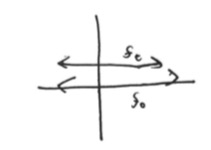
\includegraphics[width=0.30\paperwidth]{vaar2020/difftop/week06/stableEx2}
  \end{center}
  $f \in \mathcal{T}$ but $F(x,t)=(x,t)$ wich is smooth. Then if $t\neq 0, f_t(\R^1)= \{(x,t) | x\in \R \}$ is disjoint from $x$-axis.
\end{example}

\begin{example}
  $\mathcal{ T} = \{ S^1 \to \R^n | f \transv \{(x,0)| x\in \R^2 \} \}$ is stable.
\end{example}

\begin{theorem}
  \textbf{Stability theorem}
  \newline Let $X$ be compact, and a $Z \subseteq Y$ closed submanifold. The following classes of maps are stable:
    \begin{enumerate}[(1)]
      \item Immersion $X\to Y$
      \item Local diffeomorphisms $X\to Y$
      \item Submersions $X\to Y$
      \item $f \transv Z$, $f: X \to Y$
      \item $f: X \to Y$ an embedding (this is amazing!)
      \item $f: X \to Y$ diffeomorphisms
    \end{enumerate}
\end{theorem}
\begin{proof}
  $(1) \Rightarrow (2)$ by def.
  \newline Consider $f: X \to Y$ an immersion and $F:X \times [0,1] \to Y$ a homotopy with $f_0 = f$. Must find $\varepsilon>0 $ so $\forall t < \varepsilon , f_t : X\to Y$ immersion.
  \newline The idea is $(Df_t)_x: T_xX \to Tf_t(x)Y$
  \newline We know that in some coords around $(x,0) \in X \times [0,1]$, (basically looks like $u \times [0, \varepsilon), x \in u\subseteq X$ open).
  \begin{center}
    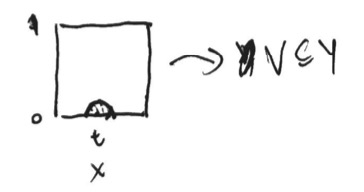
\includegraphics[width=0.30\paperwidth]{vaar2020/difftop/week06/coords}
  \end{center}
  , get coords around $f(x)\in Y, V\subseteq Y.$).
  \newline So $(Df_t)_x$ is expressible as a matrix in this open set $(Df_0)_x$ is injective if $f_0$ is an immerison. So we can capture this as there is a $k \times k$-submatrix of $(Df_0)_x$ that has nonzero determinant.
    \newline E.g. $(Df_0)_x = \begin{bmatrix}
      1 & 0 \\
      0 & 0 \\
      0 & 1
    \end{bmatrix},$ take submatrix $\begin{bmatrix}
      a_{11} & a_{12} \\
      a_{31} & a_{32}
    \end{bmatrix}$.
    \newline So write $A(x,t)$ for this submatrix of $(Df_t)_x$. If $det (A(x,t)) \neq 0 \Rightarrow $ rank of $(Df_t)_x$ is $k$, and so $Df_x$ is injective.
      \newline  So $det(A(x,t)): u \times [0, \varepsilon ) \to \R$ is a smooth function. And at our particular point $(x,0)$, $det(A(x,0))=b \neq 0$. Then $det(A(x,0)) ^{-1} \left((b-\varepsilon, b+ \varepsilon)\right)$ which is open, at these points $(Df_t)_x$ is injective. For all $x$, we get open set $u_x \subseteq X \times [0,1] $ where $(Df_t)_x$ is injective. We then know $X \times \{0\} \subseteq \cup_{c\in X}u_x$.
     Since $X \times \{0\}$ is compact a finite subcover exists, $X \times \{0\} \subseteq \cup_{i=1}^{n}u_i$.
     \newline \textbf{Modification:}
     $V_x \times [0, \varepsilon_x) \subseteq u_x$, so $V_x \subseteq X$ open.
        \begin{center}
          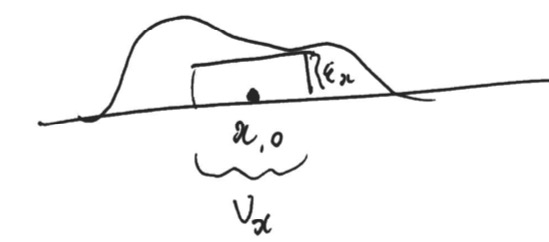
\includegraphics[width=0.30\paperwidth]{vaar2020/difftop/week06/illustr}
        \end{center}
      $X\times \{0\} \subseteq \cup_{x\in X} V_x \times [0, \varepsilon_x)$, so $X \times \{0\} \subseteq \cup_{i=1}^n V_i \times[0, \varepsilon_i)$. Conclusion $ \varepsilon = min\{\varepsilon_i | 1 \leq i \leq n \}$ then for all $t<\varepsilon Df_t$ is injective. \qedhere
\end{proof}


\section{14. feb.}
\begin{recall}
  $\mathcal{T} \subseteq C^{\infty}(X,Y)$, $\mathcal{T}$ stable if $\forall F: X \times [0,1 ] \to Y$ with $f_0 \in \mathcal{T} \Rightarrow \exists \varepsilon >0 \forall t <\varepsilon , f_{\varepsilon} \in \mathcal{T}$.
\end{recall}
$\{f: X\to Y | f \text{ a submersion }\}$ is stable when $X$ compact.
\begin{proof}
  $\forall a \in X, \exists u_{a} \subseteq X$ open neighborhood and $\varepsilon_{a}>0$, s.t. $(a,0)\in u_a \times [0, \varepsilon_a)$ that gives local coordinates, $f_0(a)\in V\subseteq Y$, s.t. $(Df_t)x$ at all $(x,t) \in u_a \times [0, \varepsilon_a)$ is represented as a matrix.
  \newline We can find an $n\times n$-submatrix of $(Df_t)x$, where $det(A(a,0))$. Now $A$ is smooth so $detA$ is smooth $\Rightarrow\exists u_a \times [0, \varepsilon_a)$ on which $det(A(x,t))\neq 0$.
    $$X\times \{0\} \subseteq \cup_{a\in X}u_a' \times[0,\varepsilon_a') \subseteq_{compact}\cup_{i=1}^{l}u_i \times [0, \varepsilon_i),$$
  and take $\varepsilon = min\{e_1, \dots, e_l \}$.
\end{proof}
